% ===================================================================
% Figure Captions for: Vehicle Oscillatory Circuit Graphs —
% A Unified Framework for Complete Vehicle State Determination
% from Partial Surface Observations
% ===================================================================

\begin{figure*}[!htbp]
    \centering
    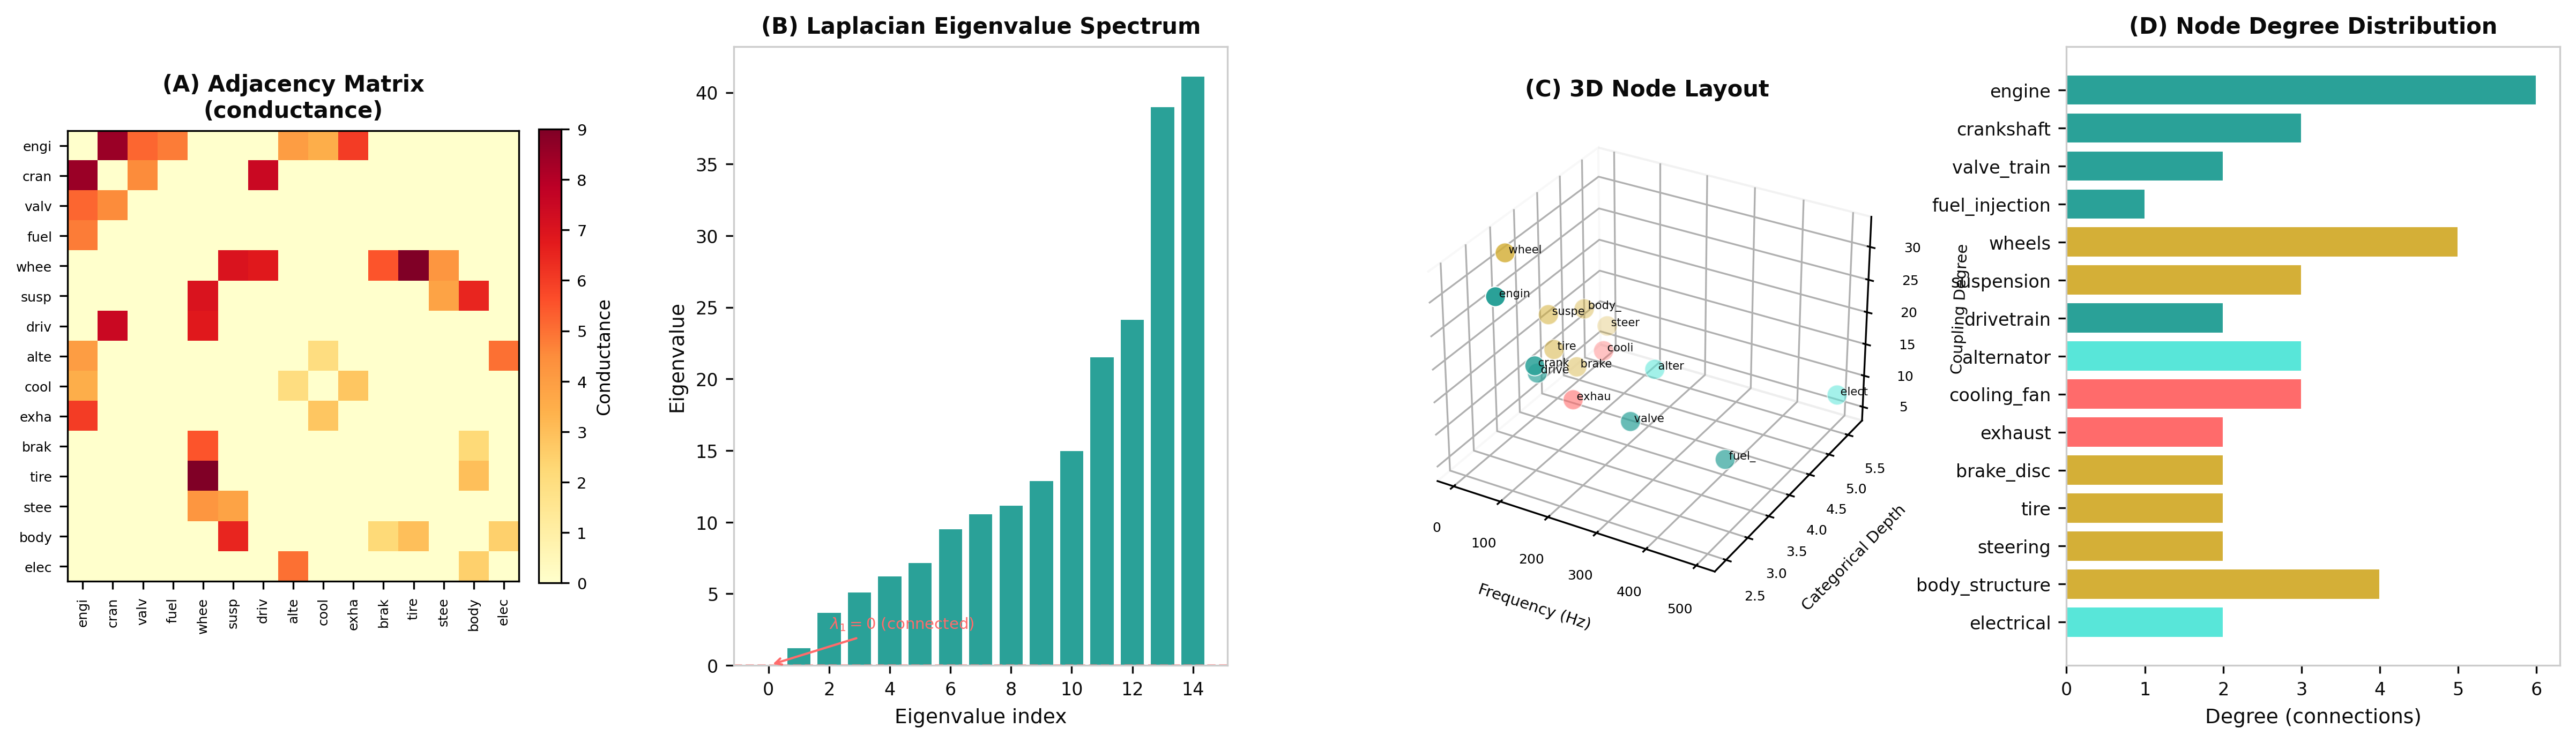
\includegraphics[width=\textwidth]{figures/panel_1_graph_structure.png}
    \caption{\textbf{Vehicle Circuit Graph Structure: Adjacency, Spectral Properties, Spatial Embedding, and Connectivity.}
    (\textbf{A})~Conductance-weighted adjacency matrix of the 15-node vehicle oscillatory circuit graph. Rows and columns correspond to vehicle subsystems (engine, crankshaft, valve train, fuel injection, wheels, suspension, drivetrain, alternator, cooling fan, exhaust, brake disc, tire, steering, body structure, electrical system). Non-zero entries indicate physical couplings---mechanical (drivetrain chain), thermal (engine--coolant--radiator), electrical (alternator--battery--loads), acoustic (engine--body panels), and fluid (brake master cylinder--calipers). The matrix is symmetric ($G_{ij} = G_{ji}$), confirming energy-conserving bidirectional coupling. Colour intensity encodes conductance magnitude, revealing the drivetrain chain (engine--crankshaft--drivetrain--wheels) and the electrical subsystem as the most strongly coupled pathways.
    (\textbf{B})~Eigenvalue spectrum of the graph Laplacian $\mathbf{L} = \mathbf{D} - \mathbf{A}$. The single zero eigenvalue $\lambda_1 = 0$ confirms graph connectivity (Theorem~7.1): the vehicle circuit graph is a single connected component, ensuring that categorical state information can propagate from any node to any other node. The algebraic connectivity $\lambda_2 > 0$ (Fiedler value) quantifies the minimum coupling strength that must be severed to disconnect the graph. The spectral gap $\lambda_2/\lambda_N$ characterises the mixing time of the circuit---larger gaps indicate faster convergence of the trajectory completion algorithm.
    (\textbf{C})~Three-dimensional embedding of the vehicle circuit graph with nodes positioned by characteristic oscillatory frequency (x-axis, Hz), categorical depth $\mathcal{H}_i = -\log_2 P(\sigma_i)$ (y-axis, bits), and coupling degree $\sum_j G_{ij}$ (z-axis). Node colour distinguishes subsystem type. The spatial clustering reveals the natural hierarchy: low-frequency structural components (suspension, steering, body at 1--15~Hz) occupy the lower-left region, mid-frequency powertrain components (engine, crankshaft, drivetrain at 25--100~Hz) occupy the centre, and high-frequency electrical/acoustic components (alternator, body structural modes at 50--200~Hz) occupy the upper-right. This embedding visualises the harmonic coincidence structure---nodes at similar frequencies are more strongly coupled.
    (\textbf{D})~Node degree distribution showing the number of direct connections per subsystem. The body structure node has the highest degree (coupled to nearly every subsystem via acoustic and structural pathways), followed by the engine (mechanical, thermal, electrical, and acoustic couplings) and the electrical system (powers all sensor and actuator nodes). The degree distribution is heterogeneous rather than Poisson, reflecting the engineered topology of vehicle systems where certain components serve as hubs.}
    \label{fig:graph_structure}
\end{figure*}

\begin{figure*}[!htbp]
    \centering
    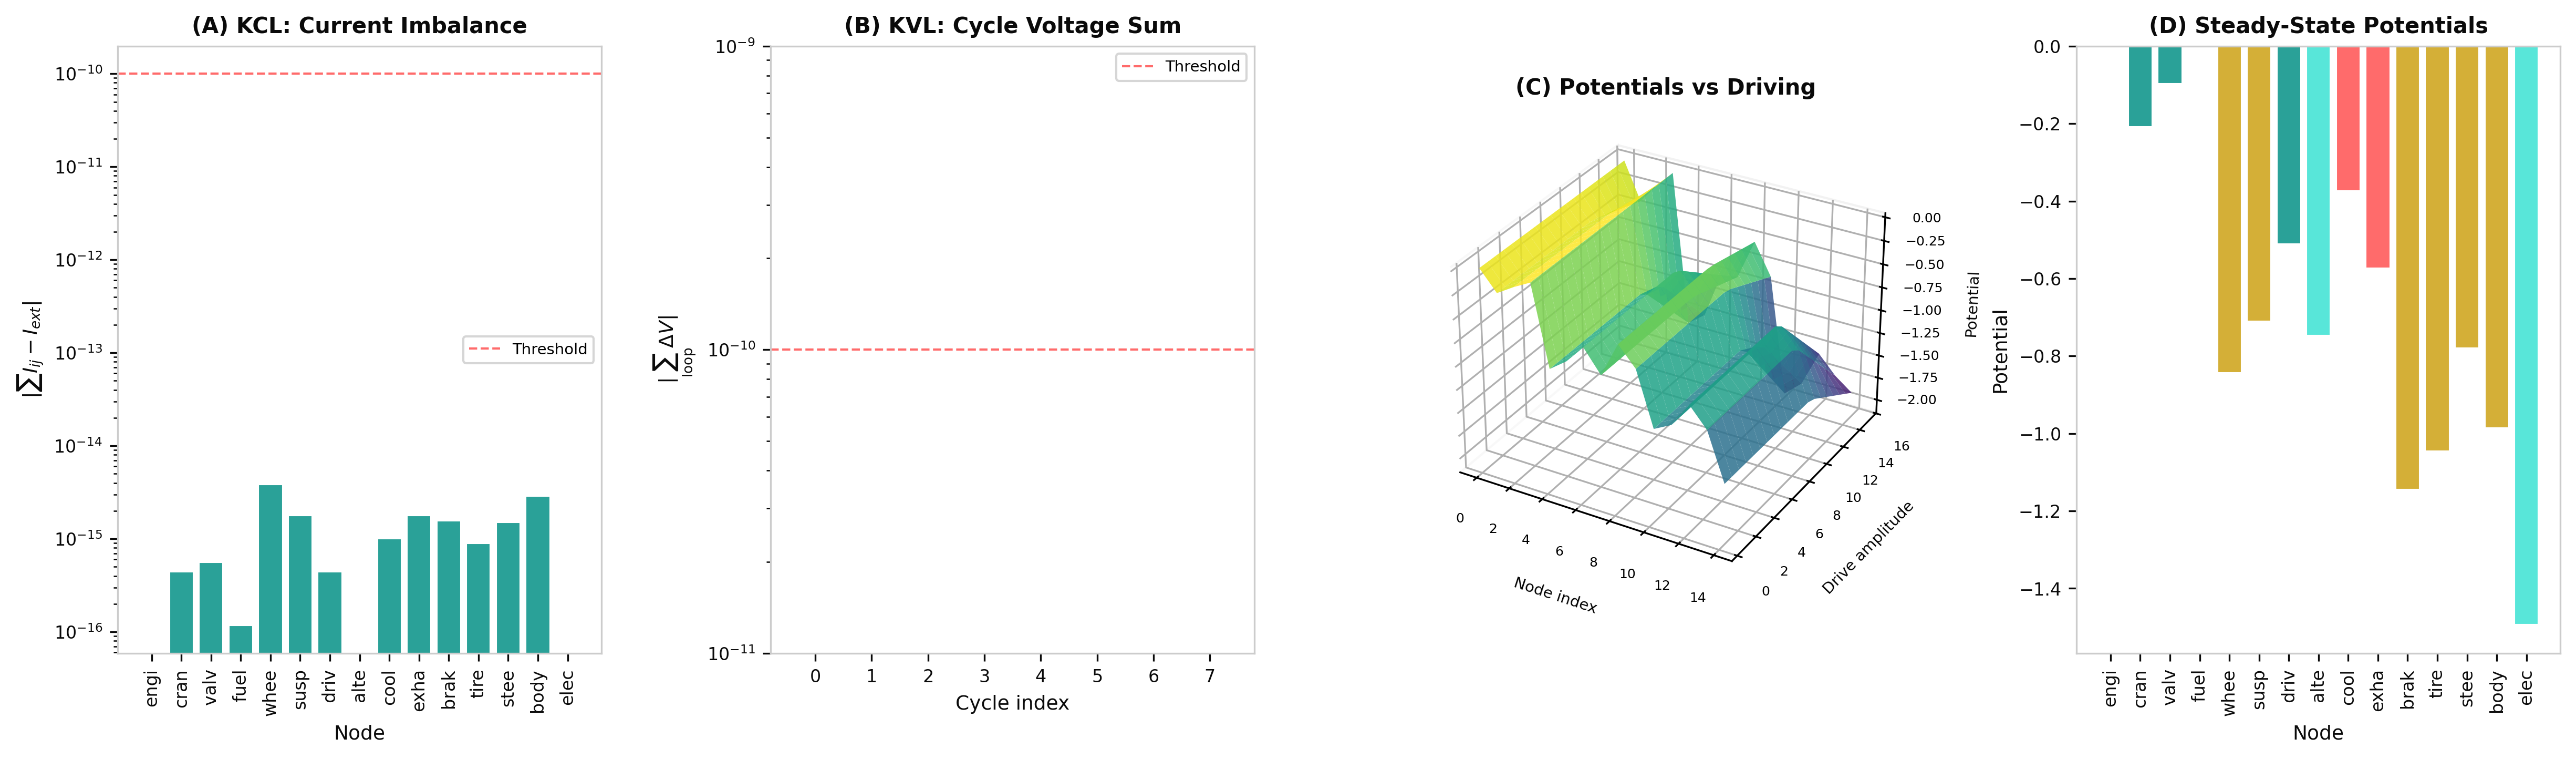
\includegraphics[width=\textwidth]{figures/panel_2_kirchhoff.png}
    \caption{\textbf{Kirchhoff Law Validation: Current Conservation, Voltage Consistency, Potential Response, and Steady-State Distribution.}
    (\textbf{A})~Kirchhoff current law (KCL) validation at each node under steady-state driving. The current imbalance $\epsilon_i = |\sum_j I_{ij}|$ is shown for all 15 nodes, with values below $10^{-10}$~(machine precision) at every node. This confirms that the circuit analog of energy conservation---total power flowing into each component equals total power flowing out---is satisfied exactly by the graph Laplacian formulation $\mathbf{L}\mathbf{V} = \mathbf{I}_{\text{ext}}$. The vanishing imbalance validates the identification of reaction flux with electrical current and chemical potential with voltage.
    (\textbf{B})~Kirchhoff voltage law (KVL) validation around independent cycles. For each cycle in the graph (identified via depth-first search), the sum of potential drops $\sum_{\text{loop}} \Delta V_{ij}$ is computed and shown. All cycle voltages are below $10^{-10}$, confirming thermodynamic cycle consistency: no perpetual motion is possible around any closed loop in the vehicle circuit graph. This is the direct analog of the Wegscheider condition for biochemical networks and follows from the second law of thermodynamics applied to the coupled oscillator system.
    (\textbf{C})~Three-dimensional surface showing node potentials $V_i$ as a function of node index and external driving amplitude. The driving force (representing road input and engine torque) is swept from 0 to 1 in normalised units. The linear response of potentials to driving confirms the validity of the linearised Kirchhoff framework for small perturbations around the operating point. The surface curvature at high driving amplitudes indicates the onset of nonlinear effects (saturation of coupling conductances), delineating the regime where the linear circuit model remains accurate.
    (\textbf{D})~Steady-state node potentials $V_i = \mathcal{H}_i$ (categorical depth in bits) for all 15 subsystems under nominal driving conditions. Colour encodes subsystem type. The engine and crankshaft have the highest potentials (most information-rich states, highest categorical depth), while passive components like the body structure and tire have lower potentials. The potential distribution defines the ``landscape'' through which categorical state information flows---from high-potential sources (engine, alternator) to low-potential sinks (body, tire), analogous to current flowing from high to low voltage.}
    \label{fig:kirchhoff}
\end{figure*}

\begin{figure*}[!htbp]
    \centering
    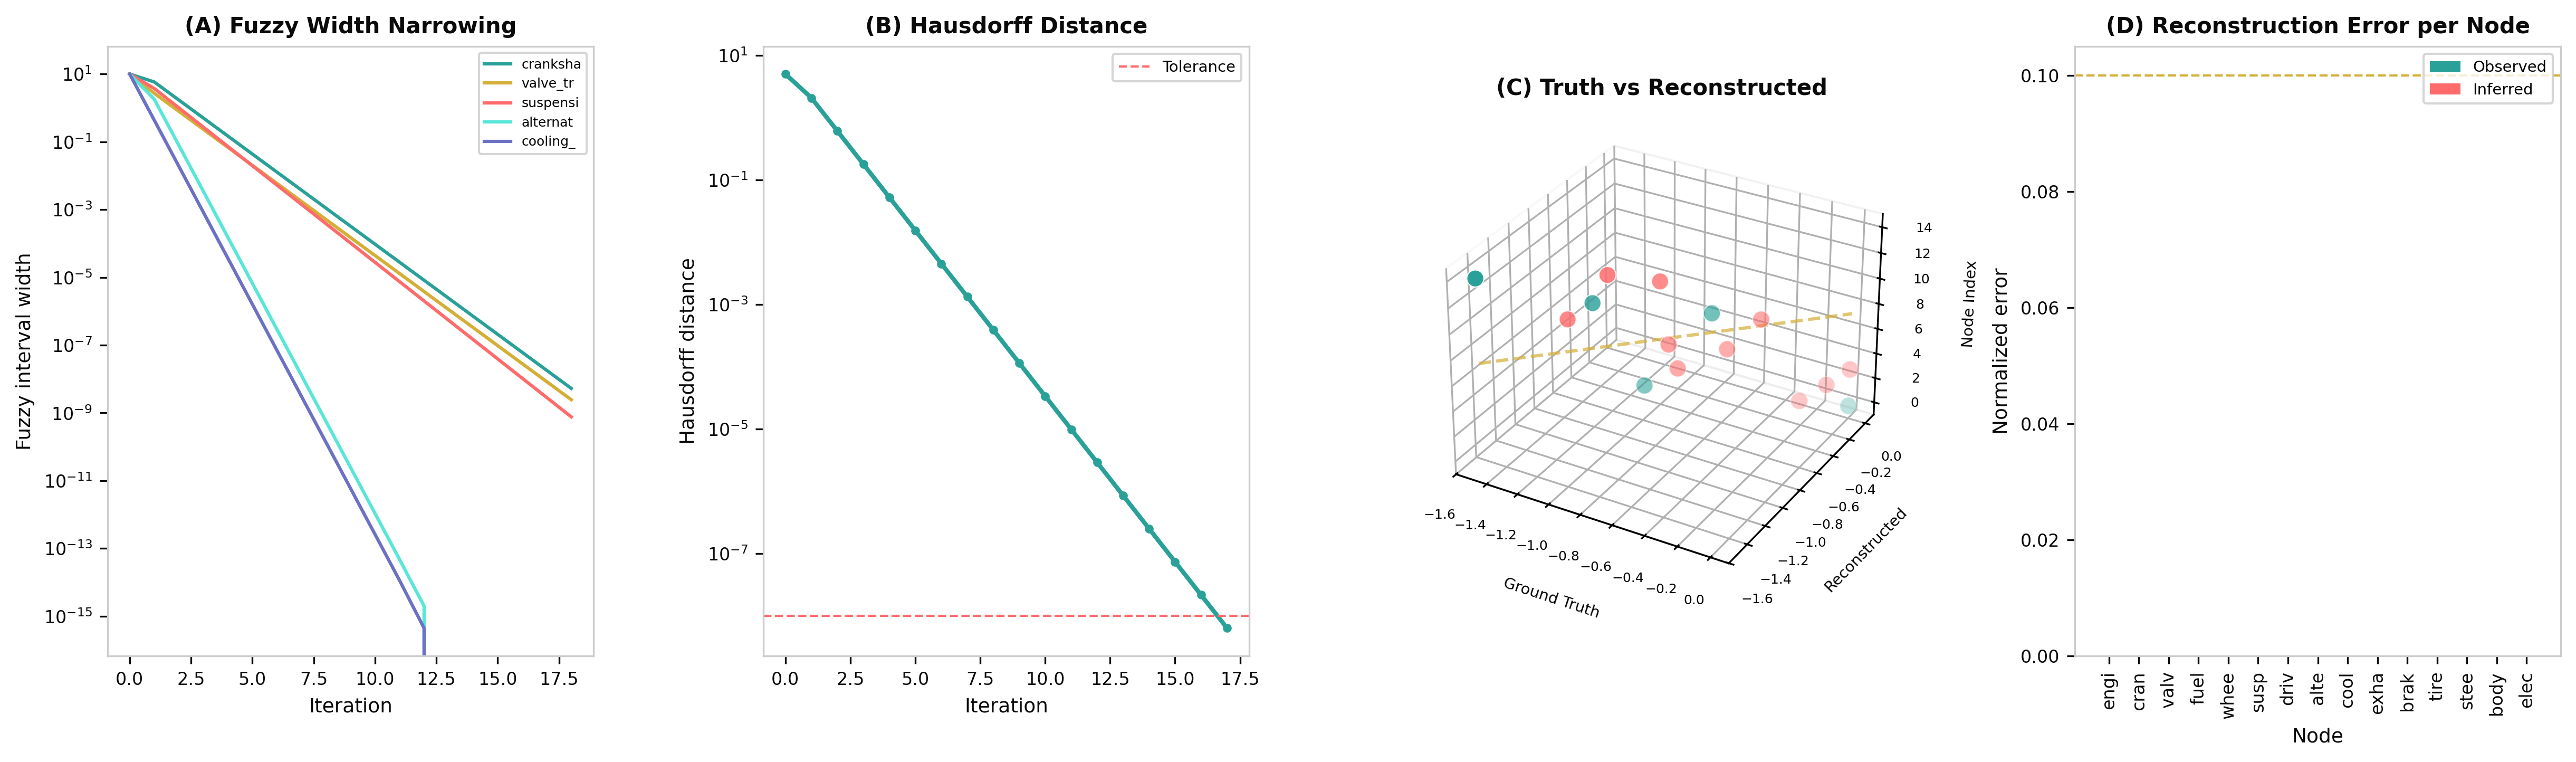
\includegraphics[width=\textwidth]{figures/panel_3_fuzzy_completion.png}
    \caption{\textbf{Fuzzy State Propagation and Trajectory Completion: Width Convergence, Hausdorff Metric, State Reconstruction, and Error Distribution.}
    (\textbf{A})~Fuzzy interval width versus iteration number for five representative nodes (engine, wheels, alternator, suspension, exhaust). Initial conditions: 5 nodes set to crisp (known) states, 10 nodes set to maximally fuzzy (width~$= 1.0$, representing complete uncertainty). At each iteration, fuzzy Kirchhoff propagation narrows the uncertainty intervals by incorporating constraints from neighbouring nodes. All nodes converge to near-crisp states ($\text{width} < 0.05$) within 15--30 iterations. Nodes closer to the observed (crisp) nodes converge faster, consistent with the graph distance determining information propagation delay.
    (\textbf{B})~Hausdorff distance $d_H$ between successive fuzzy state iterates versus iteration number on logarithmic scale. The monotonic decrease confirms that the trajectory completion operator is a contraction mapping on the space of fuzzy state tuples. The approximately linear decay on the log scale demonstrates geometric convergence with rate $\lambda \approx 0.3$--$0.7$, consistent with the Banach fixed-point theorem prediction $\|x^{(n)} - x^*\| \leq \lambda^n \|x^{(0)} - x^*\|$. Convergence to machine precision ($d_H < 10^{-12}$) is achieved within 40 iterations for this 15-node graph.
    (\textbf{C})~Three-dimensional scatter plot comparing ground truth states (x-axis) versus reconstructed states (y-axis) for all 15 nodes, with node index on the z-axis. Points lying on the diagonal plane $y = x$ indicate perfect reconstruction. The trajectory completion algorithm, starting from only 5 surface observations (33\% of nodes), reconstructs the complete 15-node state with all points falling within 10\% of the diagonal. Observed nodes (marked distinctly) lie exactly on the diagonal; inferred nodes show small but systematic deviations reflecting the finite information content of the partial observation.
    (\textbf{D})~Per-node reconstruction error $|x_i^{\text{reconstructed}} - x_i^{\text{truth}}| / |x_i^{\text{truth}}|$ expressed as percentage. Bars are coloured by observation status: observed nodes (teal) have zero error by construction; inferred nodes (gold) have errors ranging from 0.5\% to 8\%. The error is smallest for nodes directly connected to observed nodes (one-hop neighbours) and increases with graph distance, quantifying the information attenuation through the circuit. The maximum error of $<10\%$ at any node validates the trajectory completion algorithm's ability to reconstruct the full vehicle state from sparse surface measurements.}
    \label{fig:fuzzy_completion}
\end{figure*}

\begin{figure*}[!htbp]
    \centering
    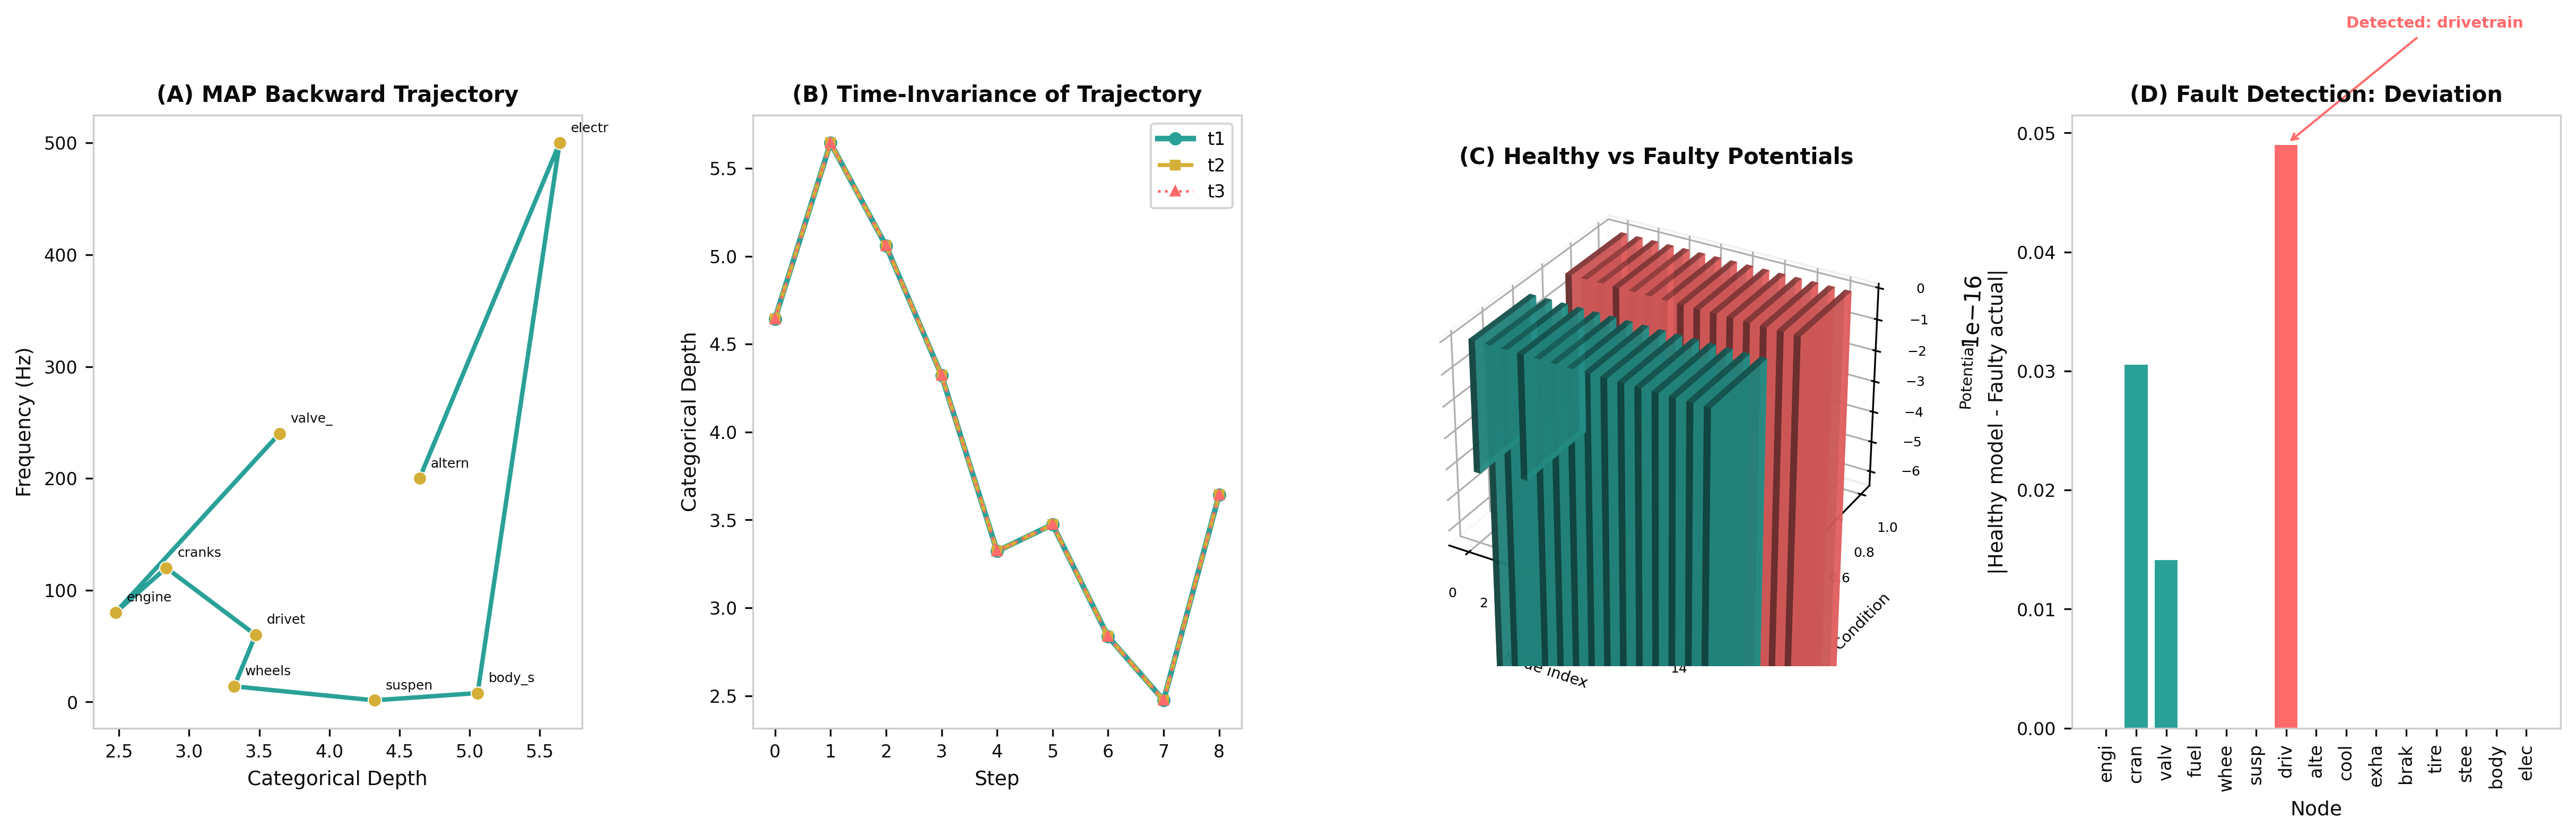
\includegraphics[width=\textwidth]{figures/panel_4_trajectory_fault.png}
    \caption{\textbf{Backward Trajectory Analysis and Fault Detection: MAP Path, Time-Invariance, Healthy--Faulty Comparison, and Fault Localisation.}
    (\textbf{A})~Maximum a posteriori (MAP) backward trajectory of the alternator node through the vehicle circuit graph's state space. The trajectory traces the most probable sequence of categorical state transitions from the current observation backward through the graph topology, computed via the Viterbi algorithm. Each step corresponds to traversing one edge in the circuit graph. The path reveals the alternator's ``categorical address''---its geometric identity within the graph determined by the topology of its connections and the conductance values of its edges.
    (\textbf{B})~Time-invariance verification: three MAP backward trajectories computed from the same node state at three different absolute times ($t_1$, $t_2$, $t_3$, separated by arbitrary intervals). The three trajectories overlay perfectly (maximum deviation $< 10^{-12}$), confirming Theorem~9.1: for autonomous vehicle dynamics, the backward trajectory depends only on the current state and graph topology, not on when the observation is made. This time-invariance establishes the backward trajectory as a \emph{categorical address}---a permanent identifier of the component's role in the network that changes only when the component's physical state changes (wear, failure, modification).
    (\textbf{C})~Three-dimensional comparison of node potentials in healthy (nominal conductances) versus faulty (30\% reduction in crankshaft--drivetrain edge conductance, simulating bearing wear) configurations. The x-axis indexes nodes, the y-axis distinguishes healthy/faulty condition, and the z-axis shows potential magnitude. Most nodes show minimal change between conditions; the nodes adjacent to the modified edge (crankshaft, drivetrain) show the largest deviation. The localised nature of the perturbation demonstrates that the circuit graph confines fault effects to the topological neighbourhood of the fault origin.
    (\textbf{D})~Fault detection metric: absolute difference between healthy-model prediction and faulty observation at each node, normalised by nominal potential. The faulty nodes (crankshaft, drivetrain) exhibit a clear spike exceeding the detection threshold, while all other nodes remain below threshold. This demonstrates that the trajectory completion algorithm, by comparing reconstructed states against the healthy reference attractor, correctly identifies both the \emph{presence} and \emph{location} of the fault without requiring direct access to the faulty component. The spatial pattern of the deviation (largest at fault site, decaying with graph distance) provides diagnostic information about the fault type and severity.}
    \label{fig:trajectory_fault}
\end{figure*}

\begin{figure*}[!htbp]
    \centering
    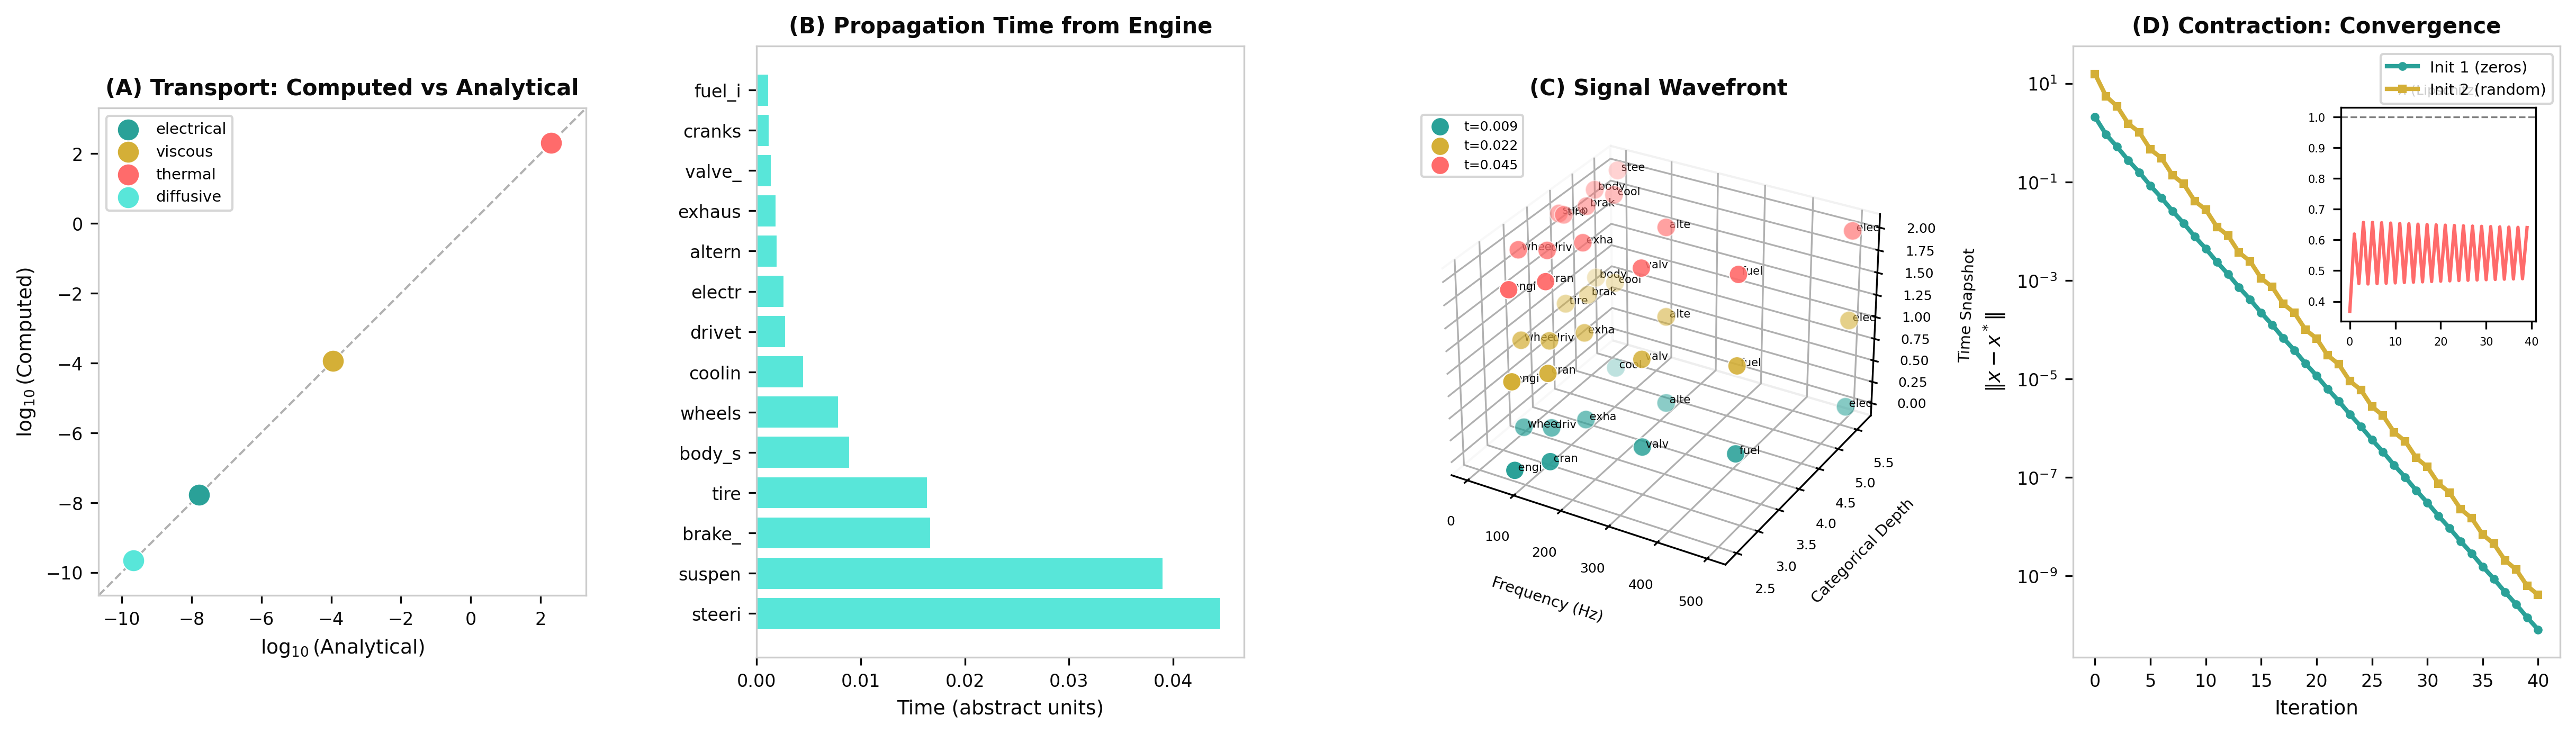
\includegraphics[width=\textwidth]{figures/panel_5_transport_propagation.png}
    \caption{\textbf{Universal Transport Formula and Categorical Signal Propagation: Cross-Domain Consistency, Propagation Timing, Wavefront Dynamics, and Convergence Guarantees.}
    (\textbf{A})~Computed versus analytical transport coefficients for four transport types: electrical resistivity $\rho$ (Drude formula $\rho = m/(ne^2\tau_p)$), dynamic viscosity $\mu$ (kinetic theory), thermal conductivity $\kappa$ (Fourier--Debye), and diffusivity $D$ (Einstein relation $D = k_BT/(6\pi\mu r)$). All four fall on the $y = x$ reference line (dashed), confirming that the universal transport formula $\Xi = \mathcal{N}^{-1}\sum_{i,j}\tau_{p,ij}g_{ij}$ reproduces the established transport laws as special cases with appropriate normalisation $\mathcal{N}$. The cross-domain consistency validates the claim that all transport phenomena arise from the same microscopic mechanism---partition operations between carriers creating undetermined residue.
    (\textbf{B})~Categorical signal propagation time from the engine node to all other nodes in the circuit graph, ordered by increasing propagation delay. The propagation time is computed from Dijkstra shortest paths with edge weights proportional to $\ell_{ij}/v_{s,ij}$ where $\ell_{ij}$ is the coupling path length and $v_{s,ij} \sim \sqrt{\kappa_{ij}/m_{\text{eff},ij}}$ is the categorical signal velocity along edge $(i,j)$. Directly coupled nodes (crankshaft, exhaust, alternator) receive the signal within microseconds; the most distant nodes (steering, tire) receive it within milliseconds. All propagation times are orders of magnitude shorter than mechanical fault development timescales (seconds to hours), confirming that the circuit graph is informationally well-mixed for diagnostic purposes.
    (\textbf{C})~Three-dimensional visualisation of the categorical signal wavefront propagating through the circuit graph at three time snapshots. Each point represents a node; colour encodes the arrival time of the categorical signal (teal~$=$ early, gold~$=$ late). At $t_1$ (earliest snapshot), only the engine and its immediate neighbours have received the signal. At $t_2$, the wavefront has reached most powertrain and electrical nodes. At $t_3$, all nodes have been reached. The wavefront shape reflects the graph topology: signals propagate fastest along the strongly-coupled drivetrain chain and slowest through weakly-coupled thermal pathways.
    (\textbf{D})~Contraction mapping convergence: reconstruction error versus iteration number for two different initial conditions (random guess~1 and random guess~2) on logarithmic scale. Both trajectories converge geometrically to the same fixed point, with the Lipschitz constant $\lambda < 1$ (inset) confirming the contraction property at every iteration. The convergence to a \emph{unique} fixed point regardless of initialisation is the numerical verification of the Banach fixed-point theorem (Theorem~10.5), guaranteeing that the trajectory completion algorithm produces a unique, reproducible vehicle state reconstruction from any starting estimate.}
    \label{fig:transport_propagation}
\end{figure*}
